\section{Do the Explanations Hold Up?}
\label{sec:evaluation}

\subsection{How explanations can be tested}
Agreement with expectations does not show that an explanation reflects the model. \textit{Faithfulness} tests ask whether the features a method marks as important actually drive the output. Deletion tests remove top-ranked inputs and track the predicted probability. ROAR removes them and retrains, which avoids the distribution shift of plain deletion \cite{hooker2019benchmark}. Sanity checks randomise model weights or labels, which should destroy a faithful map; Adebayo \textit{et al.} showed that some popular saliency methods barely change \cite{adebayo2018sanity}. Simulated EEG with known class-relevant signals provides a ground truth that real data lack \cite{ravindran2023empirical}.

These tests matter for EEG. Cui \textit{et al.}~\cite{cui2023towards} compared seven attribution methods against random maps on three datasets, including the Cao subset. Gradient$\times$input, DeepLIFT, integrated gradients and LRP beat the random baseline, whereas saliency maps, deconvolution and guided backpropagation mostly did not. Even the better methods produced misleading maps for some samples: deleting the channel marked most important raised one prediction from 0.6 to 0.98. Their study covers gradient-based methods and two shallow networks, so it does not settle the question for CAM, SHAP or attention, which most reviewed papers use.

\subsection{Appraisal of the 27 studies}
Fig.~\ref{fig:appraisal} shows the result. Twenty-one studies report explanations that at least partly agree with known physiology, but this is the weakest check. For eye-state tasks the agreement holds by definition, and several claims rest on a few chosen images.

Only one study tested faithfulness quantitatively: Feng \textit{et al.}~\cite{feng2025id3rsnet} used perturbation sensitivity and deletion tests, comparing against one other model without a random baseline. Seven studies applied a partial check, of three kinds. \textit{Plausibility} measures whether maps land where expected \cite{saxena2026lowlight,rafy2026domain}. \textit{Consistency} compares methods or resamples: SHAP against partial dependence on the same model ($r = 0.849$) \cite{hasan2024validation}, selection stability across folds \cite{jiang2026eeg}, and bootstrap aggregation \cite{puspasari2026predicting}. \textit{Sufficiency} shows that top-ranked features retrain to a similar score \cite{vitorino2023adversarial,zhou2021predicting}. These checks are useful, but none shows that the explanation reflects what the model does. Agreement between two methods on one model is consistency, and a stable feature can still be a shortcut. The remaining 19 studies did not evaluate the explanation.

Only 11 of the 27 studies clearly tested on unseen drivers, and a further three state it without enough detail to verify. Three share code, all from one research group. Only one study combines a faithfulness test with testing on unseen drivers \cite{feng2025id3rsnet}, and its authors still read alertness partly as muscle and drift signals. Passing a faithfulness test does not rule out a shortcut.

\begin{figure}[!t]
\centering
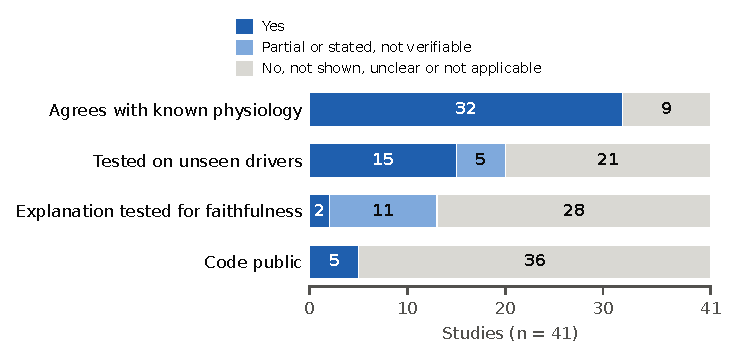
\includegraphics[width=\columnwidth]{fig2_appraisal}
\caption{Appraisal of the 27 detection studies on four checks. Counts describe the examined set, not the whole field; per-study ratings are in Tables~\ref{tab:eeg}--\ref{tab:vision}.}
\label{fig:appraisal}
\end{figure}

\subsection{Accuracy depends on the test scheme}
An explanation of a model that has memorised its test drivers has limited value, so the test scheme bears directly on RQ3. Fig.~\ref{fig:validation} plots reported accuracy by scheme. The median is 97.5\% under random or within-subject splits and 77.1\% on unseen drivers. The tasks and datasets differ, so this comparison is only descriptive, but the same pattern appears within single studies: 96.9\% to 50.8\% for Seo \textit{et al.}~\cite{seo2025driver}, 97.47\% to 85.43\% for Zhou \textit{et al.}~\cite{zhou2026sedriven}, and 97.2\% to 92.4\% for Rafy \textit{et al.} when moving to another dataset \cite{rafy2026domain}. On UTA-RLDD, a subject-independent baseline reached 65.2\% at video level, with human observers at 57.8\% \cite{ghoddoosian2019realistic}; later papers report about 97\% on the same data with image-level splits, although on a simpler two-class task \cite{rafy2026domain}.

The effect is not uniform. In Hasan \textit{et al.}~\cite{hasan2024validation}, leave-one-participant-out reached 80.1\%, close to a single hold-out split (81.3\%) and above their noisy 10-fold results, on a small dataset of 156 observations. Variance also matters: subject-level means can hide failure on individual drivers, such as the 47.3\% worst case behind a 90.7\% mean in Nomura \textit{et al.}~\cite{nomura2025drowsiness}. Several EEG results also report the best epoch selected on test-fold accuracy \cite{cui2022eeg,cui2022compact,cui2021subject,feng2025id3rsnet}, which is mildly optimistic.

\begin{figure}[!t]
\centering
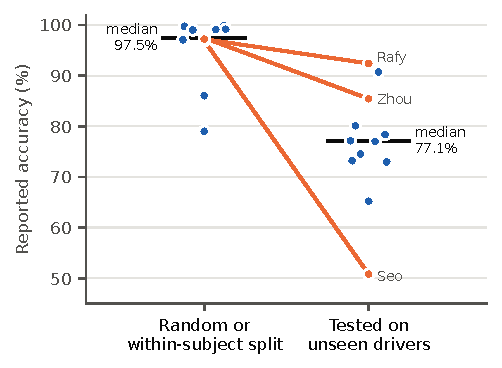
\includegraphics[width=\columnwidth]{fig3_validation}
\caption{Reported accuracy by test scheme, descriptive only because tasks differ. Orange lines join results from one study. Left: \cite{seo2025driver,zhou2026sedriven,gao2025idsrn,alarnaout2025exploiting,mcdonald2014steering,rafy2026domain,florez2023cnn,florez2024realtime,hassan2025realtime,albadawi2023realtime,ersoy2026improving}. Right: \cite{cui2022eeg,cui2022compact,cui2021subject,feng2025id3rsnet,seo2025driver,jiang2026eeg,zhou2026sedriven,hasan2024validation,puspasari2026predicting,rafy2026domain,nomura2025drowsiness,ghoddoosian2019realistic}. Studies with unverifiable splits are omitted.}
\label{fig:validation}
\end{figure}

\subsection{Explanations inherit the label}
Labels limit what any explanation can mean. Four recurring problems appear in the reviewed set.

\textit{Labels derived from model inputs.} AlArnaout \textit{et al.}~\cite{alarnaout2025exploiting} label windows using heart-rate change and level, while mean RR, the inverse of heart rate, is an input. Albadawi \textit{et al.}~\cite{albadawi2023realtime} generate labels from thresholds on the same eye, mouth and head features the classifier receives. High accuracy then partly measures whether the model can recover the rule.

\textit{Eye state as drowsiness.} When the label is open versus closed \cite{florez2023cnn,florez2024realtime,hassan2025realtime,ersoy2026improving}, a heatmap on the eye confirms the definition.

\textit{Time on task as fatigue.} Labels from session order \cite{puspasari2026predicting} or task stage \cite{jiang2026eeg} cannot separate fatigue from anything else that changes over a session.

\textit{Eye signals in the input and the label.} PERCLOS labels combined with EOG input or without eye-artefact removal \cite{zhang2024multimodal,zhou2026sedriven,gao2025idsrn} may let a model detect eye closure directly. Zhou \textit{et al.} raise this risk themselves and test it through frontal-channel removal \cite{zhou2026sedriven}.

By contrast, McDonald \textit{et al.}~\cite{mcdonald2014steering} use video-rated drowsiness with a steering-only model, and Nomura \textit{et al.}~\cite{nomura2025drowsiness} and Ghoddoosian \textit{et al.}~\cite{ghoddoosian2019realistic} use ratings independent of the model's computed features. These give their explanations a firmer footing.

\subsection{Case study: testing one interpretable model and its explanations}
\label{sec:casestudy}
Published accuracy for interpretable EEG models often assumes a protocol that a vehicle cannot follow. Cui \textit{et al.} note that their compact model's batch normalisation uses the whole test subject at once, and that about 6\% of its accuracy depends on this \cite{cui2022compact}. We measured the effect on the multi-channel InterpretableCNN \cite{cui2022eeg}, using our own implementation of its training recipe on the balanced 11-subject subset (2{,}022 samples) under leave-one-subject-out, with five seeds.

Table~\ref{tab:casestudy} shows the results. With statistics from the whole held-out subject, the model reaches 77.93\%, close to the published 78.35\%. Scoring windows one at a time with the same design, as a live system must, gives a constant output (50.00\%, AUC 0.498). Training with running statistics restores a usable streaming model at 73.68\%, which is 4.25 points below the whole-subject figure (better on 9 of 11 subjects for the whole-subject protocol, Wilcoxon $p = 0.042$). On all 27 subjects of the original dataset, using our own conversion of the data, the streaming model reaches 73.59\% balanced accuracy and an AUC of 0.828, so the figure is not specific to the subset.

For comparison, the deep model DeltaGateNet reports 83.21\% on this subset with subject-level five-fold splits \cite{po2026deltagatenet}. Under leave-one-subject-out we obtained 64.74\%, but this is a single seed and a different split, so it is preliminary and is not a direct replication.

\textit{Attribution tests.} We then tested explanations of the two InterpretableCNN variants on every held-out window (five seeds, 11 subjects; all tests across subjects are two-sided Wilcoxon signed-rank tests). Retraining reproduced the accuracies in Table~\ref{tab:casestudy} exactly. We compared saliency, gradient$\times$input, integrated gradients (zero baseline, 50 steps) and CAM with CNN-Fixation tracing, the method published with this model \cite{cui2022eeg}, each explaining the logit margin of the predicted class with normalisation statistics held fixed. The peripheral channel set and the frequency bands were fixed before any results were seen. Code and per-subject results are at \url{https://github.com/sunnyyadav3339/Driver-Drowsiness-Detection-from-EEG}. \todo{True only after research/ is pushed.}

\textit{The decision depends on other windows.} A heatmap explains one window, but under whole-subject normalisation the decision also depends on the driver's other windows. Table~\ref{tab:context} measures this by rescoring the same windows with the same weights and changing only the statistics; labels were used only to build the contexts. Statistics from 30 random windows nearly reproduce the whole-subject result, with 4.80\% of predictions changing. Statistics from alert windows alone change 24.55\% of predictions and raise the predicted-drowsy share from 45.59\% to 68.21\%, and the maps drift far from the baseline (similarity 0.502). A sample-level heatmap shows none of this dependence.

\textit{Faithfulness and sanity can disagree.} Table~\ref{tab:faith} and Fig.~\ref{fig:xaitests} show that every method beat random deletion on at least 10 of 11 subjects ($p \le 0.002$), including the published tracing method, which the EEG comparison of Cui \textit{et al.}~\cite{cui2023towards} did not evaluate. Gradient$\times$input and integrated gradients were strongest under point deletion. This result needs caution: in a nearly piecewise-linear network, removing the points with the largest positive first-order contribution should lower the margin almost by construction, and zeroing takes EEG outside its normal distribution. Channel deletion is more conservative, and there the gap narrows (0.50 against 0.56 for tracing). The same two methods are the weakest on the sanity check: their maps keep a rank correlation of about 0.51 with maps from a randomly initialised network, against 0.13 for saliency and 0.17 for tracing. Multiplying by the input carries amplitude structure into the map whatever the weights are, as Adebayo \textit{et al.} caution \cite{adebayo2018sanity}. Saliency beat random here, unlike in Cui \textit{et al.}~\cite{cui2023towards}, although the procedures differ. No method wins on every test, so reporting one test alone can mislead. Maps were also only moderately stable: channel maps from identical data and different seeds correlated at 0.56 for tracing and 0.72--0.75 for the others.

\textit{What the model uses.} Fig.~\ref{fig:xaitests}(c) and Fig.~\ref{fig:scalp} give the all-window picture for the whole-subject model. Removing theta, alpha or delta lowered P(drowsy) by 0.24, 0.17 and 0.09 on all 11 subjects ($p = 0.001$), and zeroing the 15 central channels lowered it by 0.41. This supports the drowsy reading. Spatially, tracing also agrees with the published alert reading: it placed 64.0\% of alert relevance on the 15 peripheral channels against 45.6\% for drowsy ($p = 0.007$), peaking at F7 for alert and at PZ and CPZ for drowsy. Gradient$\times$input shows a smaller difference (51.9\% against 46.2\%, $p = 0.010$).

On this subset, perturbation does not confirm the alert reading. Zeroing the peripheral channels barely changed P(alert) ($-0.007$, $p = 0.58$), and removing beta had no significant effect ($+0.008$, $p = 0.28$); only gamma removal lowered it, slightly ($-0.036$, $p = 0.001$). Across all windows of this subset, the model behaves like a detector of central low-frequency evidence, with alertness close to the absence of that evidence plus a small high-frequency contribution. Results for the running-statistics variant are similar. These findings qualify the artefact reading but do not refute it. Removing signal also lowers its energy, which may itself favour the alert class. Muscle activity is broadband, so band removal cannot isolate it, and averages can hide windows that behave as the published examples do. The analysis covers one model and 11 subjects, and we did not correct for multiple comparisons, so it should be treated as descriptive evidence.

\textit{The full dataset gives a clearer answer.} We repeated the removal tests with the running-statistics model on all 27 subjects of the original dataset, using our own conversion with natural class balance (five seeds, labelled trials from the 31st of each session). Zeroing the peripheral channels lowered P(alert) by 0.110 ($p < 0.001$), and removing gamma lowered it by 0.074 ($p < 0.001$). The artefact reading therefore has more support on the full dataset than on the 11-subject subset. Here too, removing theta lowered P(drowsy) most among the bands (0.244). The general point stands: a conclusion drawn from inspected samples should be tested across all windows, and here both the test and the choice of data change the conclusion.

\begin{table}[!t]
\centering
\caption{Same Windows and Weights, Different Normalisation Statistics (Whole-Subject Model; Mean over 11 Subjects and 5 Seeds)}
\label{tab:context}
\footnotesize
\begin{tabularx}{\columnwidth}{@{}YL{0.8cm}L{1.15cm}L{1.1cm}L{1.0cm}@{}}
\toprule
\textbf{Statistics from} & \textbf{Acc. (\%)} & \textbf{Changed (\%)} & \textbf{Predicted drowsy (\%)} & \textbf{Map sim.} \\
\midrule
All windows of the subject & 77.93 & 0.00 & 45.59 & 1.000 \\
30 random windows & 77.55 & 4.80 & 45.39 & 0.890 \\
Alert windows only & 68.65 & 24.55 & 68.21 & 0.502 \\
Drowsy windows only & 72.12 & 14.59 & 31.02 & 0.694 \\
\bottomrule
\end{tabularx}
\end{table}

\begin{table}[!t]
\centering
\caption{Attribution Tests on InterpretableCNN. Del.: Area Under the Deletion Curve (Lower Is Better); Sanity: Spearman Correlation with a Randomised Model (Lower Is Better); Stab.: Correlation Across Seeds (Higher Is Better)}
\label{tab:faith}
\footnotesize
\begin{tabularx}{\columnwidth}{@{}YL{0.85cm}L{0.95cm}L{0.8cm}L{0.7cm}@{}}
\toprule
\textbf{Method} & \textbf{Del., points} & \textbf{Del., channels} & \textbf{Sanity} & \textbf{Stab.} \\
\midrule
\multicolumn{5}{@{}l}{\textit{Whole-subject statistics}} \\
CAM + tracing & 0.542 & 0.561 & 0.174 & 0.563 \\
Saliency & 0.580 & 0.641 & 0.128 & 0.754 \\
Gradient$\times$input & 0.185 & 0.501 & 0.513 & 0.719 \\
Integrated gradients & 0.178 & 0.500 & 0.515 & 0.730 \\
Random & 0.667 & 0.707 & -- & -- \\
\midrule
\multicolumn{5}{@{}l}{\textit{Running statistics}} \\
CAM + tracing & 0.563 & 0.584 & 0.167 & 0.603 \\
Saliency & 0.583 & 0.659 & 0.126 & 0.800 \\
Gradient$\times$input & 0.152 & 0.526 & 0.510 & 0.770 \\
Integrated gradients & 0.161 & 0.525 & 0.511 & 0.775 \\
Random & 0.695 & 0.737 & -- & -- \\
\bottomrule
\end{tabularx}
\end{table}

\begin{figure*}[!t]
\centering
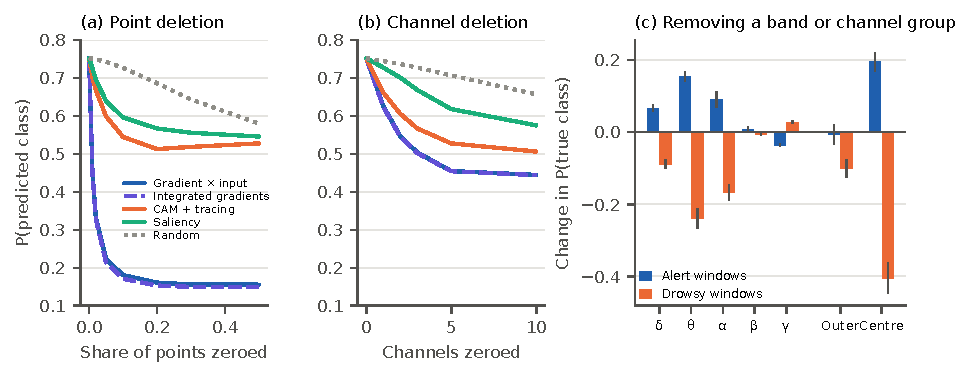
\includegraphics[width=\textwidth]{fig4_xai_tests}
\caption{Tests on the whole-subject model, every held-out window. (a), (b) Probability of the originally predicted class as the top-ranked points or channels are zeroed. (c) Change in the probability of the true class when a frequency band is removed or the 15 outer (peripheral) or 15 central channels are zeroed; bars show the mean over subjects, whiskers the standard error.}
\label{fig:xaitests}
\end{figure*}

\begin{figure}[!t]
\centering
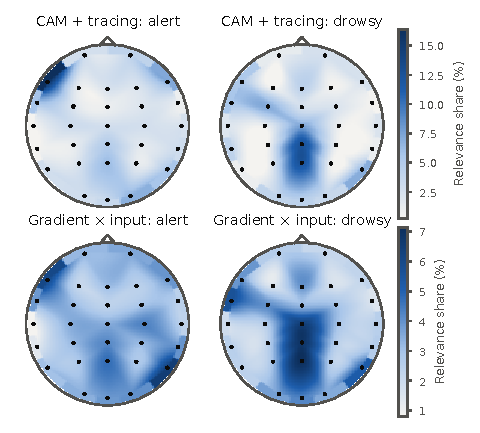
\includegraphics[width=\columnwidth]{fig5_scalp}
\caption{Share of positive relevance per channel for the whole-subject model, averaged over every held-out window per class, then over seeds and subjects. Each method has its own colour scale. Electrode positions are approximate.}
\label{fig:scalp}
\end{figure}

\begin{table}[!t]
\centering
\caption{Case Study on the 11-Subject Subset, Leave-One-Subject-Out}
\label{tab:casestudy}
\footnotesize
\begin{tabularx}{\columnwidth}{@{}YL{1.0cm}L{0.9cm}L{0.8cm}@{}}
\toprule
\textbf{Model and protocol} & \textbf{Acc. (\%)} & \textbf{AUC} & \textbf{Seeds} \\
\midrule
InterpretableCNN, normalised over whole test subject & 77.93 & 0.835 & 5 \\
InterpretableCNN, same, scored one window at a time & 50.00 & 0.498 & 5 \\
InterpretableCNN, running statistics, one window at a time & 73.68 & 0.818 & 5 \\
Band power + logistic regression, one window at a time & 67.14 & 0.743 & 1 \\
DeltaGateNet, one window at a time (preliminary) & 64.74 & 0.766 & 1 \\
EEGNet, one window at a time & 63.85 & 0.752 & 5 \\
\bottomrule
\end{tabularx}
\end{table}
